\documentclass{article}

\usepackage{amssymb}
\usepackage{amsmath}
\usepackage{mathtools} 
\usepackage{graphicx}
\usepackage{geometry}
\usepackage{longtable}
\usepackage{multirow}
\usepackage{lscape}
\usepackage{booktabs}
\usepackage{bbold}
\usepackage{chngcntr}

\counterwithout{figure}{section}
\counterwithout{table}{section}

\setlength{\parindent}{0pt}
\geometry{a4paper}

\newcommand{\E}{\mathbb{E}}
\newcommand{\N}{\mathcal{N}}
\newcommand{\1}{\mathbb{1}}
\DeclareMathOperator{\sign}{sign}
\DeclareMathOperator{\mean}{mean}
\DeclareMathOperator{\var}{var}
\DeclareMathOperator{\sd}{sd}
\DeclareMathOperator{\cov}{cov}
\DeclareMathOperator{\corr}{corr}
\DeclareMathOperator{\Prob}{Prob}

\title{Transitional Dynamics in Growth Model with Skill Mismatch}
\date{\today}
\author{Rong Fan}

\begin{document}
\maketitle
\begin{abstract}
I develop a model with endogenous growth and on the job search, while workers and firms are heterogeneous in terms of the skill and technology and level. Higher skill level and technology level generate higher output; however, difference between technology and skill level introduces penalty of mismatch due to the specialization of the task. The mismatch penalty term could be important for the economic growth, since it increases the incentive for the worker to take the training to catch up with the technology change (firms to adopt new technology to adjust to the skill change); but it could at the same time decrease the overall efficiency and introduce uneven wage growth for different skill group. 
\end{abstract}

\clearpage
\section{Introduction}
There are two engines of economic growth: technology and human capital. Higher technology and human capital level increases the productivity of the economy, but the growth could be unbalanced. It's important to study the interaction between the technology and the human capital, especially with the increasing complementarity between these two factors of production. 

\clearpage
\section{Related Literature}

\subsection{Labor Market Trends}
Violante(2002)\cite{Violante2002} provides a quantitative theory to study the effects of technological acceleration on wage inequality. The acceleration reduces worker's capacity to transfer skills from old to new machines, generating a rise in the cross-sectional variance of skills, and therefore of wages.
Acemoglu and Autor(2011)\cite{AcemogluAutor2011} study the change in return to skill (job polarization) using a task-based framework, the change of wage can be a result of technology change favoring one type of worker (low, median or high skill); or machinery substituting certain kinds of job tasks (routine cognitive). In this paper, they also documented the labor market trend from 1963 to 2010 mainly using data from CPS and Census data, while occupations are evaluated using DOT and O*NET. The main trend of the labor market can be summarized as following: (1) Wage premium decreased at first during 1970s, and increased afterward until now. (2) Different wage groups grew evenly before 1970s, but the wage of the low wage group started to decrease while the wage of higher wage group started to increase faster while during 1980s and mid-1990s; after the period of uneven growth, the low wage group started to catch up and the high wage group continued to grow (job polarization). 
Akerman et al.(2015)\cite{Akermanetal2015} discuss how the adoption of broadband internet affects different type of workers. By using employer-employee data and internet data from Norway, and the public program as an exogenous treatment, they find that broadband internet improves the labor market outcomes and productivity of skilled worker, but worsens that of unskilled workers. 
Barany and Zsofia(2018)\cite{BaranyZsofia2018} emphasize that polarization is a long-run phenomenon and closely linked to the shift from manufacturing to services and explicitly model the sectoral choice of workers.

\subsection{Innovation and Technology Adoption}
Some papers focus on the process of innovation, how the new ideas are generated and how the firms make the decision to invest in R\&D. 
Kortum (1997)\cite{Kortum1997} develops a search-theoretic model to study the technological change process. Ideas arrive to the researchers as a Poisson process, its efficiency is drawn from a probability distribution which depends on the research effort stock. The technological frontier is generated by all the past research, and will determine the productivity. 
Comin et al.(2006)\cite{Cominetal2006} incorporate R\&D and technology adoption in RBC model to understand the medium-term cycles. This framework can generate procyclical R\&D investment and adoption intensities, which explains the persistent response of economic activity to the high frequency fluctuations. 
Acemoglu et al.(2013)\cite{Acemogluetal2013} develop a model of endogenous reallocation and innovation with heterogeneous firms, they estimate parameters of the model using US Census micro data on firm-level output, R\&D and patenting. Unskilled workers are used in the production, while skilled workers perform R\&D functions and operations. Firms differ in terms of their innovative capacities, they choose their investment level on R\&D. 
Aghion et al.(2014)\cite{Aghionetal2014} survey Schumpeterian growth theory, in which new innovations replace older technologies, resulting in endogenous growth, individuals can choose to allocate the labor supply between production and research. The theory provides us a framework to study macroeconomic growth while incorporating many microeconomic issues regarding incentives, policies and organizations that interact with growth.
Atkeson et al.(2019)\cite{Atkesonetal2019} nest several canonical models into one unifying model with endogenous technology adoption. Production labor hours are used to produce the intermediate good; research labor hours are used to produce the research good. Final good is a CES aggregate of the intermediate goods, intermediate good producers need to invest research good in order to enter the market, to develop new product, or to upgrade the technology. The new entries can enter the market producing new products or replacing the incumbents. \\

Some papers focus on the technology adoption. When the new technologies are invented, how would the firms make the decision to put the new technology into production. 
Hall and Khan (2003)\cite{HallKhan2003} discuss the technology diffusion when facing uncertainty of benefits and costs, the demand for new technology is mainly determined by the skill level of workers and the technical capacity, customer commitment and network effects. 
Michelacci et al.(2007)\cite{Michelaccietal2007} incorporate labor market search frictions and technology adoption in Solow growth model, the technology could be neutral or investment-specific, the newly created job will directly adopt the technology at the frontier, while the old job can only upgrade the technology to the frontier with certain probability. They find that advancements in the neutral technology lead to an increase in job destruction, job reallocation, and unemployment. 
K{\"o}nig et al.(2016)\cite{Konigetal2016} develop a dynamic growth model where the firm can innovate to increase the productivity or imitate other firm's technology. 
Anzoategui et al.(2019)\cite{Anzoateguietal2019} develop a model with an endogenous TFP mechanism that allows for costly development and adoption of technologies. Innovators use skilled labor to create new intermediate goods, adopters use skilled workers to convert unadopted technologies into ones that can be used in production; the slow recovery could be explained by the sharp decline in adoption intensity during the Great Recession. \\

The innovation and technology adoption can generate endogenous growth in the economy. 
Luttmer(2012)\cite{Luttmer2012} identifies the assumptions needed to guarantee a balanced growth path with stationary firm distribution. Firms differ in their productivity level $z$, optimizing their production size. New firms can enter with certain hazard rate by paying a cost, they will start their business with an exogenous growing productivity level $Z_t$, which drives up the equilibrium wage level (by labor market clearing condition). Incumbents are facing permanent productivity shocks (BM) and will leave the market if the productivity is lower than certain threshold, since they will not be able to afford the fixed cost to maintain their business. If entrants can enter with technology level slightly better than the technologies used by the least productive incumbents, the economy can sustain a balanced growth path with stationary firm distribution (Zipf's law).
Perla and Tonetti(2014)\cite{PerlaTonetti2014} develop an analytically tractable model where firms at the bottom of the productivity distribution can imitate more productive firms. Firms are heterogeneous in terms of their productivity, there is no aggregate or individual exogenous growth, no idiosyncratic productivity shocks, and there is no enter and exit. The only dynamic is that each period, firms make the search decision with the opportunity cost of current period production, they can redraw their productivity level from the current distribution if they decide to search. The growth is endogenous, at each period, firms with productivity under certain threshold would decide to search; and they redraw productivity from the the part of the distribution above this threshold, since all firms below the threshold would be searching without producing. BGP would be achieved with geometric growth rate, starting with an initial Pareto distribution with certain conditions satisfied. 
Benhabib et al.(2017)\cite{Benhabibetal2017} study how the interaction between adoption and innovation determines the shape of the productivity distribution, the expansion of the technology frontier, and the aggregate economic growth rate. Firms can adopt the technology to increase their productivity by paying a cost, they can also choose to innovate and charge the licensing fee. 
Akcigit et al.(2018)\cite{Akcigitetal2018} bring together the knowledge diffusion models and innovation based growth models. Skilled research workers produce innovations, unskilled labor are used in production.  Productivity of skilled workers evolve endogenously over time as a result of endogenous interactions or exogenous external learning. Workers choose the meeting rate with others, when they meet, they group into research team, and the innovation quality depend on the leader's productivity and the number of members. They use the European Patent Office data to estimate the model.  \\

\subsection{Human capital}
Mincer (1974)\cite{Mincer1974} develops earnings equations which is the potential earning minus the investment cost in human capital, the potential earning depends on the year of schooling and work experience, the human capital investment linearly declines in work experience. 
Barron and Black (1989)\cite{BarronBlack1989} use survey data to test the effect of on-the-job training, the training has significant effect on wage and productivity growth. \\

The accumulation of human capital takes two forms. Firstly, the knowledge will be passed across generations through education, labor can get their initial skill level by choosing the schooling investment. Secondly, the human can be increased during the life time through learning-by-doing (the experience will be accumulated by doing the job) or learning-or-doing (workers need to spend time to learn new skills with the opportunity cost of production). 
Kalemli-Ozcan et al.(2000)\cite{Kalemli-Ozcanetal2000} develop a continuous time, overlapping generations model in which individuals make optimal schooling investment choices facing certain probability of death, workers only invest in education at the beginning of their lives, and work until the death. 
Galor and Moav (2004)\cite{GalorMoav2004} develop a growth model with overlapping generation, individuals acquire their human capital in the first period, which is a function of the education expenditure; individuals start to work in the second period, and allocate their wage income. The economy growth is driven by physical capital accumulation at the beginning, then human capital at the later stage. 
Imai et al.(2004)\cite{Imaietal2004} build a dynamic life cycle model where the agents choose optimal consumption and labor supply, and human capital evolves depending on the amount of labor supply. They use NLSY79 data to estimate the intertemporal elasticity of substitution in labor supply, and get the elasticity much larger than the estimation in micro literature. 
Bohacek and Kapicka (2008)\cite{BohacekKapicka2008} set up a dynamic private information model where the workers can increase their human capital by investing schooling time. Individuals are heterogeneous in terms of their ability, which is private information for them; in each period, they allocate their time between work, leisure and human capital accumulation.  \\

Burdett et al.(2011)\cite{Burdettetal2011} incorporates learning-by-doing and life cycle in the BM model, workers are heterogeneous in terms of productivity and accumulate experience while working. The wage variance could be decomposed into workers' heterogeneity, firms' heterogeneity, difference in experience and sorting. 
kapicka and Neira (2013) studies a life-cycle economy with risky human capital accumulation. Agents live for J periods, their earnings are determined by ability, human capital and labor supply, the ability is constant and is known from the beginning, human capital can be accumulated by learning with idiosyncratic shock; agents dislike working and learning. 
Stantcheva (2015)\cite{Stantcheva2015} builds a dynamic model where the workers can allocate their time between working and training, and training can increase the worker's human capital stock. The training and working could be substitute (learning or doing) or complement (learning and doing). 
Stantcheva (2017)\cite{Stantcheva2017} set up a life cycle model with risky human capital. Agents live for T periods, each period, agents can build their stock of human capital by spending money; wage rate is determined by the human capital stock and stochastic ability. \\

\subsection{Interaction between technology and human capital}
The technology and human capital are complementary component in the production, so the investment decision will depend on the level of the other component. 
Redding(1996)\cite{Redding1996} discusses the strategic game between workers and entrepreneurs on decisions of human capital and R\&D investment under the context of an endogenous growth model. 
Beaudry et al.(2006)\cite{Beaudryetal2006} use the city level data to study the interaction between technology adoption and labor market conditions. Compared with the old technology, the new technology uses a different form of capital, and is skilled biased; the new technology is more productive than the old technology only when used with a high fraction of skill workers. The empirical results show that cities with a high fraction of college educated workers adopted PCs more intensively; and cities adopting PCs intensively witnessed greater increases in returns to skill. 
Ad{\~a}o et al.(2020)\cite{Adaoetal2020} develop a theory to study technological transitions driven by both worker
reallocation within a generation and changes in the distribution of skills across generations. New born workers choose their skill type to maximize the expected future earning less the cost; then with fixed skill type, workers choose to work in high-tech or low-tech sector.  \\

The interaction between technology and skill is important for the economic growth. 
Lloyd-Ellis and Roberts(2002)\cite{Lloyd-EllisRoberts2002} develop an endogenous growth model with skill acquisition and innovation, skills are required to implement and invent new technology. The economic growth only takes the form of growth of variety in the CES production function of final good. A sustainable growth could be maintained only when technology and skill grow at the same rate. If skill grows too slow, higher technology won't be able to put into production and no labor would be available for R\&D. If technology grows too slow, the workers won't have the incentive to spend time in school, since they cannot benefit from specialization when no higher technology is available.
Stokey(2014)\cite{Stokey2014} develops a growth model in which heterogeneous firms invest in R\&D and heterogeneous workers invest in human capital. By assuming that the cost of R\&D and skill investment is scaled by the firm's or the worker's own surplus, and homothetic CES production function, the balanced growth path is easy to solve. All the firms and workers will choose the same rate of growth, and the relative skill-technology position and match will stay constant. The only parameters that capture the growth are the cost of investments for R\&D and human capital, which jointly determine the growth rate of the economy. 
Luttmer(2015)\cite{Luttmer2015} summarizes four models of knowledge diffusion and long-run growth with different ways to model long-run evolution of skill distribution, and discussed different possible distribution that could be used the describe the growth process. The distribution evolves through three channels: (1) producers could learn from each others (social learning) but with some search delay and learning delay; (2) the productivity state evolves according to Brownian motion with time trend; (3) producers under certain threshold would exit the market and redraw from the current distribution. What happens in the long run depends on initial conditions.
Stokey(2020)\cite{Stokey2020} develops a model in which economic growth comes from technology and skill acquisition; while growth can take 2 forms: higher TFP and more variety. Due to the complementarity between technology and skill, the endogenous growth would happen only if both parts grow at the same time. TFP growth mainly depends on worker's incentive to acquire new skill, determined by the parameters capturing the skill growth rate. With high skill growth rate, firms have the incentive to increase their technology since the marginal gain would be high; with low skill growth rate, firms would switch to variety growth. Variety growth mainly depends on the firm's incentive to enter and stay in the market, determined by the difference between parameters capturing technology and skill growth; high variety growth could suppress TFP growth since it dilutes profit of each individual firm and reduce the technology adoption and skill acquisition incentive. 

\section{Search Model with heterogeneous firms and workers}
In this section, I build a dynamic search-theoretic model of the labor market in which the match quality is decided jointly by the worker's skill and the firm's technology. This model is an extension of MPV (2018)\cite{MPV2018}, in which the match quality is endogenous and decided jointly by the worker and the firm.
To model the mismatch, I adopted the framework of Lise and Postel-Vinay (2015)\cite{LisePostelVinay2015}. 

\subsection{Environment}
Time $T = 1, 2, 3 \dots$ is discrete and continues forever, the economy is populated by a continuum of risk neutral workers with measure 1. Both workers and firms maximize their present value of income or profit, with discount rate $\beta$. Firms produce a single, homogeneous, non storable numeraire consumption good, using only labor. \\

\textbf{Production function: }
Production function is a function of aggregate productivity($z$), labor skill($a$) and firm's technology level ($b$). The production is higher with a higher $z$, $a$ and $b$ in general, however, there is a penalty associated with the skill mismatch, the production would be lower if the worker's skill level is too far away from the firm's requirement. 
\begin{align*}
f(z,a,b) &= z[\kappa a^{\frac{\sigma-1}{\sigma}}+(1-\kappa) b^{\frac{\sigma-1}{\sigma}}]^{\frac{\sigma}{\sigma-1}}-1\{a<b\}\frac{\alpha_u(b-a)^2}{a}
\end{align*}
$\kappa$ is the output share of worker's skill, while $1-\kappa$ is the output share of firm's technology level.  $\sigma$ is the elasticity of substitution between firm's technology and worker's skill. If the worker is under-qualified ($a<b$), the firm receives a mismatch penalty $\alpha_u(b-a)^2$ since the worker is not able to complete all the tasks of the job. \\

If the worker is over-qualified ($a<b$), the worker will receive the disutility $d(a,b)$.  
\begin{align*}
d(a,b) &=\alpha_o\frac{(a-b)^2}{a}
\end{align*}
\textbf{Worker: }
Workers are heterogeneous in terms of their skill level $a_i$, they get their initial skill level from distribution $\Gamma_a$. 
Each period, regardless of his employment status, with probability $P_a$, the worker receives a shock on his skill level. 
Also, the worker can decide if he wants to invest in his human capital by taking the on-the-job training. \\

At the beginning of each period, each worker will receive an idiosyncratic shock for home production/utility shock for leaving the Labor Force (LF), noted by $\epsilon_n$, which is drawn from Pareto distribution. The worker will receive unemployment insurance$b_u$ if he is unemployed and stays in the LF, wage $\omega(z,a,b',b)$ (explained later) if he is employed and stays in the LF, and $\epsilon_n$ if he choose to leave the LF. If the worker leaves the LF, he will not be matched to any firms during the period, and he will be automatically unemployed next period. \\
\begin{align*}
\epsilon_n &\sim Pareto(\theta_n^{\frac{1}{\lambda_n}}b_u,\lambda_n) \\
\E \epsilon_n &= \frac{\lambda_n}{\lambda_n-1}\theta_n^{\frac{1}{\lambda_n}}b_u \\
\Prob &\{\epsilon_n > b_u\} = \theta_n
\end{align*}

\textbf{Firm: }
Firms are heterogeneous in terms of their technology level $b_j$. When a firm firstly enter the market, he draws his type from distribution $\Gamma_b$.  
Each period, with probability $P_b$, the firm receives shock on his technology level. 
Also, after entering the market, the technology level of the firm will start to depreciate, firms will need to pay a cost to adjust their technology level. 

\subsection{Search and Match}
The match is random. All the unemployed workers $u$ and share $s$ of the employed workers are searching. With probability $\delta$, the match is destroyed exogenously, so the number of employed workers searching for a new job is $s(1-\delta)e$. Firms pay a fixed cost $K$ to create and advertise the vacancy. The effective job market tightness is a function of vacancy created $\nu$ and workers actively searching of the job $u+s(1-\delta)e$. 
\begin{align*}
\theta = \frac{\nu}{u+s(1-\delta)e}
\end{align*}
The matching function is assumed to be Cobb-Douglas, the job arriving rate $\phi$ is assumed to be a function of the market tightness as following. 
\begin{align*}
\phi_t(\theta) = \Phi \theta_t^\alpha
\end{align*}

\subsection{Value of not-in-labor-force, unemployment and employment }
The value of not in the labor force is $V_n(\epsilon_n)$ depending on the home productivity received by the worker; the value of unemployment is $V_u$, it's constant for all the workers. The total output of the match is noted as $P(z,a,b)$, which is the expected value of the match's total production; the over-qualification disutility is noted as $D(z,a,b)$, which is the expected value of total disutility the worker may receive; the net surplus of the match is noted as $S(z,a,b)$, which is $P(z,a,b)$ subtracted by $V_u$ (opportunity cost) and $D(z,a,b)$ (disutility). They are all depend on TFP $z$, worker's skill level $a$ and firm's technology level $b$. The value of employment (contract) is $V_e(z,a,b',b)$, which depends on not only TFP $z$, worker's skill level $a$ and firm's technology level $b$, but also the bargaining power of the worker related to his employment history $b'$. 

\subsection{Wage determination}
The wage is determined by Bertrand competition, the worker accumulate bargaining power during the employment. When firstly enter the labor market, the worker does not have any bargaining power, the value of the contract will only be $V_u$, since it's the minimum value the firm needs to deliver in order to have the worker accept the job. If the worker is not over-qualified ($a \leq b$), the actual payment would be the same as the value of contract $V_u$; if the worker is over-qualified ($a<b$), the actual payment needs to be $V_u+D(z,a,b)$, since the firm needs to compensate the extra disutility the worker receive.  \\

With probability $s\phi(\theta_t)$, the worker will meet new employer and gain bargaining power while the employers compete over the worker. If the worker meet a new match with technology level $b'$, which generates higher surplus $S(z,a,b')>S(z,a,b)$, the new employee needs to promise at least how much the old employee is able to deliver, which is $S(z,a,b)$, in order to win the auction, the worker will choose to jump to the new match, and the value of new contract is $V_e(z,a,b,b') = S(z,a,b)$, the bargaining power is $(S(z,a,b)-V_u)/(S(z,a,b')-V_u)$. If the worker meet a new match which generates lower surplus, there are 2 cases. If the maximum value the new match can deliver to the worker is less than the worker's current contract value, then nothing would change; otherwise, the old employee will pay at least how much the new employee is able to afford to keep the worker, the worker will stay in the old job with a promotion, the value of contract will increase to $V_e(z,a,b',b) = S(z,a,b')$, and the bargaining power will be increased to $(S(z,a,b')-V_u)/(S(z,a,b)-V_u)$. Similar with the previous cast, if the worker is underqualified, the actual payment is the same as the contract $V_e(z,a,b,b')$; if the worker is overqualified, the firm needs to compensate the disutility the worker would receive $V_e(z,a,b,b')+D(z,a,b)$. If the worker get separated endogenously or exogenously from the job, the worker lose all the bargaining power, and will have to start to climb on the wage ladder again. \\

If the worker newly enters the labor market, his current value is $V_u$, then when he get a match $S(z,a,b')$: 
\begin{table}[h!]
\centering
\begin{tabular}{llc}
\hline \hline
New match \\
Surplus & Contract & Bargaining power \\
\hline
$S(z,a,b') \leq V_u$ &Stay unemployed & \\
$S(z,a,b')>V_u$ &$V_e(z,a,0,b) = V_u$ & 0\\
\hline \hline
\end{tabular}
\end{table}

If the worker is already employed, the surplus of the match is $S(z,a,b)$, while his current value of contract is $V_e(z,a,b'',b) = S(z,a,b'')$ with a current bargaining power $S(z,a,b'')/S(z,a,b)$, then when he get a match $S(z,a,b')$: 
\begin{table}[h!]
\centering
\begin{tabular}{lll}
\hline \hline
New match \\
Surplus & Contract & Bargaining power \\
\hline
$S(z,a,b')<V_e(z,a,b'',b)$ & $ V_e(z,a,b'',b)=S(z,a,b'') $ & $S(z,a,b'')/S(z,a,b)$ \\
$S(z,a,b') \in (V_e(z,a,b'',b),S(z,a,b))$ & $V_e(z,a,b',b)=S(z,a,b')$ & $S(z,a,b')/S(z,a,b)$\\
$ S(z,a,b')>S(z,a,b)$ &$ V_e(z,a,b,b')=S(z,a,b)$ & $S(z,a,b)/S(z,a,b')$ \\
\hline \hline
\end{tabular}
\end{table}
\subsection{Worker's and firm's decision}
\subsubsection*{Worker} 
Workers decide if they want to search for new job, then they decide if they want to sign the contract if they get a new match, they also make the human capital investment decision. \\

\textbf{Search: }
Firstly, all workers need to decide if they want to stay in the LF or not. If the worker is unemployed, then the worker will leave the LF if $V_n(\epsilon_n)>V_u$; if the worker is employed, then the worker will leave the LF if $V_n(\epsilon_n)>S(z,a,b)$. $V_u$ is the value function for being unemployed; $V_n(\epsilon_n)$ is the value function for being not in the labor force; $S(z,a,b)$ is the surplus generated by the match.\\

\textbf{Contract: }
Secondly, if an unemployed worker searches for job and get matched , he needs to decide take or reject the offer; if an employed worker searches for job and get matched, he needs to decide which contract to accept, from the old employee or from the new match. The unemployed worker will accept the job if $\bar{V}_e(z,a,b_u,b) > V_u$; the employed worker will accept the new job if $\bar{V}_e(z,a,b') > \bar{V}_e(z,a,b)$. $\bar{V}_e(z,a,b)$ is the value of contract offered by the firm. \\

\textbf{Human Capital: }
Thirdly, the worker makes the decision on the human capital investment to maximize the joint value of the match. Once the match if formed, they can choose their skill level by paying an adjustment cost if their choice is different from their current skill level. The adjustment cost is convex in the difference, the more they want to adjust, the more expensive the cost would be. 

\subsubsection*{Firm}
Firms firstly need to decide if they want to open a vacancy and enter the market; while entering, they have the opportunity to choose their initial technology level by paying a start-up cost. After being matched, they decide if they want to pay a cost to adjust their technology. \\

\textbf{Vacancy opening: }
Firms pay the cost associated with vacancy creation and posting to enter the market.  \\

\textbf{Technology adoption: }
There are 2 ways to adopt the technology. When entering the market, firms can pay a start-up cost to choose their initial technology level, the cost is increasing in adjustment they make. After entering the market, once the match if formed, they can choose the technology level, while paying an adjustment cost convex in the difference. 

\subsection{Timing of Events}
\begin{enumerate}
\item Nature draws the $\epsilon_t$ innovation to TFP $z_t \sim AR(1)$, and firms and workers observe the realization of the productivity shock. 
\item Idiosyncratic shocks are realized on firms' technology and workers' human capital. 
\item Idiosyncratic shocks on home production are realized, both employed and unemployed decide if they want to stay or leave the labor force. 
\item Firms and workers produce. Firms pay the workers wage $\omega(z,a,b',b)$ according to their state-contingent contract. Unemployed workers receive the unemployment benefit $b$. Agents not in the LF receive the home production benefit. 
\item Existing matches break up: firstly by endogenous separation if the firms or workers can be better off by destroying the match, secondly by exogenous separation with probability $\delta$. When the workers get separated from the firms, they can not search during the current period, they will be part of the unemployed workers and start to search starting from next period. 
\item Human capital of unemployed workers depreciates. Technology depreciates.
\item Firms enter the market and make the vacancy posting decision. When they enter the market, they pay the cost associated with vacancy creation and posting and initial technology adoption. They don't know their type $b$, they only know the distribution of $b$ from which they will draw their type from later on depending on their initial choice. Firms can observe perfectly the distribution of workers while making the decision. 
\item Firms are randomly matched to previously unemployed workers and a share $s$ of the skill employed workers. At the same time, the firm type $b$ is revealed. 
\item Upon meet, firms offer contract to theirs matched workers. If the worker is unemployed, the firm will offer a take-it-or-leave-it contract; if the worker is already employed, his current employee and the new matched firm, while they can observe each others' type perfectly, will Bertrand-compete in contract. 
\item Unemployed worker will decide to take the contract or not, employed worker will decide which contract to take. 
\item After the match is successfully formed, workers and firms have the opportunity to increase their skill and technology level by paying an adjustment cost. 
\end{enumerate}

\section{Equilibrium}
In the Benchmark model, I consider the case where both skill and technology depreciation rate $\delta_a = \delta_b = 0$. Cost of training for workers $\phi_a \to \infty$, while cost of technology adoption for firms $\phi_b \to \infty$. I also assume that there is no aggregate shocks on TFP, while there is no idiosyncratic shocks on the skill level and the technology level ($P_a = P_b = 0$). 

\subsection{Value function}
For unemployed worker, when they are matched to a firm, the firm will only promise to deliver a minimum value $V_{u,t}$ to make the worker indifferent between staying unemployed and taking the job. So the value of being unemployed is independent of time and state. The worker always have the choice to leave the LF and get $V_{n,t}(\epsilon_n)$ depending on the shock realized, since the shocks are iid distributed, both $V_n(\epsilon_n)$ and $V_u$ are state independent. 
\begin{align*}
V_{u,t} &= b_u+\beta\E_t\max\{V_{u,t+1},V_{n,t+1}(\epsilon_n)\} = V_u \\
V_{n,t}(\epsilon_n) &= \epsilon_n+\beta\E_t\max\{V_{u,t+1},V_{n,t+1}(\epsilon_n)\} = V_{n}(\epsilon_n) 
\end{align*}
We can drop the time index and solve $V_u$ and $V_n(\epsilon_n)$: 
\begin{align*}
V_u &= b_u+\beta\E\max\{V_u,V_n(\epsilon_n)\} \\
V_n(\epsilon_n) &= \epsilon_n+\beta\E\max\{V_u,V_n(\epsilon_n)\}  \\
\max\{V_u,V_n(\epsilon_n)\} &= \max \{V_u,\epsilon_n\}+\beta\E\max\{V_u,V_n(\epsilon_n)\}  \\
\E\max\{V_u,V_n(\epsilon_n)\} &= \E\max \{V_u,\epsilon_n\}+\beta\E\max\{V_u,V_n(\epsilon_n)\}  \\
\E\max\{V_u,V_n(\epsilon_n)\} &= \frac{1}{1-\beta}\E\max \{b_u,\epsilon_n\}  \\
\E\max \{b_u,\epsilon_n\}  &= (1-\theta_n)b_u+\int_{b_u}^{\infty}\frac{\lambda_n(\theta_n b_u)^{\lambda_n}}{x^{\lambda_n}}dx \\
										&= (1-\theta_n)b_u+\frac{\lambda_n}{\lambda_n-1}(\theta^{\frac{1}{\lambda_n}}b_u)^{\lambda_n}b_u^{1-\lambda_n} \\
										&= (1+\frac{\theta_n}{\lambda_n-1})b_u \\
V_u &= b_u+\beta(1+\frac{\theta_n}{\lambda_n-1})\frac{b_u}{1-\beta}\\
V_n(\epsilon_n) &= \epsilon_n+\beta(1+\frac{\theta_n}{\lambda_n-1})\frac{b_u}{1-\beta} 
\end{align*}
$V_u$ and $V_n(\epsilon_n)$ are linear in $b_u$ and $\epsilon_n$, the unemployed worker will leave the labor force when $\epsilon_n>b_u$. Value function $V_u$ and $V_n(\epsilon_n)$ are decreasing in $\lambda_n$. \\

Output of the match $f(a,b)$ is a function of worker's skill level and firm's technology level, it is the net output $g(a,b)$ minus the mismatch penalty $p(a,b)$ if the worker is underqualified. If the worker is overqualified, then the worker will receive a disutility $d(a,b)$. 
\begin{align*}
f(a,b) &= g(a,b)-p(a,b) \\
g(a,b) &= [\kappa a^{\frac{\sigma-1}{\sigma}}+(1-\kappa) b^{\frac{\sigma-1}{\sigma}}]^{\frac{\sigma}{\sigma-1}} \\
p(a,b) &= 1\{a<b\}\alpha_u\frac{(b-a)^2}{a}\\
d(a,b) &= 1\{a>b\}\alpha_o\frac{(b-a)^2}{a}
\end{align*}

The total surplus $S(a,b)$, the expected net output $P(a,b)$ and the expected disutility $D(a,b)$ of the match could be solved as: 
\begin{align*}
S(a,b) &= f(a,b)-d(a,b)+(1-\delta)\beta \E\max\{\E\max\{S(a,b),\epsilon_n\}-\E\max\{b_u,\epsilon_n\},0 \}  \\
P(a,b)
&= \begin{dcases}
f(a,b)+(1-\delta)\beta(\E\max\{S(a,b),\epsilon_n\}-\E\max\{b_u,\epsilon_n\}+d(a,b)), \quad  \max\{S(a,b),\epsilon_n\}>\E\max\{b_u,\epsilon_n\} \\
f(a,b), \quad \max\{S(a,b),\epsilon_n\}<\E\max\{b_u,\epsilon_n\}
\end{dcases} \\
D(a,b) &=P(a,b)-S(a,b)
\end{align*}

In order to solve the total total surplus, we need to solve $\E\max\{S(a,b),\epsilon_n\}$ and $\E\max\{V_u,V_n(\epsilon_n)\}$. Also, notice that the employed worker will leave the labor force if he receives home production shock $\epsilon_n>\epsilon^*(a,b)$, while $\epsilon^*(a,b) = S(a,b)$. 
\begin{align*}
\epsilon^*(a,b)\leq\theta_n^{\frac{1}{\lambda_n}}b_u, \quad \E\max\{\epsilon^*(a,b),\epsilon_n\} &= \frac{\lambda_n}{\lambda_n-1}\theta^{\frac{1}{\lambda_n}}b_u \\
\epsilon^*(a,b)>\theta_n^{\frac{1}{\lambda_n}}b_u, \quad \E\max\{\epsilon^*(a,b),\epsilon_n\} &= (1-(\frac{\theta_n^{\frac{1}{\lambda_n}}b_u}{\epsilon^*(a,b)})^{\lambda_n})\epsilon^*(a,b)+\int_{\epsilon^*(a,b)}^{\infty}\frac{\lambda_n(\theta_n b_u)^{\lambda_n}}{x^{\lambda_n}}dx \\
												&= \epsilon^*(a,b)+\frac{\theta_n}{\lambda_n-1}b_u^{\lambda_n}{\epsilon^*(a,b)}^{1-\lambda_n} \\		
\E\max\{b_u,\epsilon_n\} &= b_u +\frac{\theta_n}{\lambda_n-1}b_u 
\end{align*}	
$\max\{\E\max\{S(a,b),\epsilon_n\}-\E\max\{b_u,\epsilon_n\},0 \} $ can be solved as: 
\begin{align*}
&\max\{\E\max\{S(a,b),\epsilon_n\}-\E\max\{b_u,\epsilon_n\},0 \}   \\
&= \begin{dcases}
0 & ,f(a,b) \leq b_u \\
\epsilon^*(a,b)-b_u +\frac{\theta_n}{\lambda_n-1}b_u^{\lambda_n}({\epsilon^*(a,b)}^{1-\lambda_n}-b_u^{1-\lambda_n}) & ,f(a,b)>b_u 
\end{dcases}
\end{align*}	
So when the technology adjustment cost $\phi_b \to \infty$, $S(a,b)$ can be solved as:
\begin{align*}
S(a,b) 
&= \begin{dcases}
f(a,b)-d(a,b) & ,f(a,b)  \leq b_u \\
f(a,b)-d(a,b)+(1-\delta)\beta(\epsilon^*(a,b)-b_u +\frac{\theta_n}{\lambda_n-1}b_u^{\lambda_n}({\epsilon^*(a,b)}^{1-\lambda_n}-b_u^{1-\lambda_n})) & ,f(a,b)>b_u 
\end{dcases}
\end{align*}	

The value function for total surplus with different $\lambda$ is plotted in figure \ref{Analytical1}. With different $\lambda$, the decision rule for accepting the job is the same, the unemployed worker will accept the job when $\E\max\{S(a,b),V_n(\epsilon_n)\}>\E\max \{V_u,V_n(\epsilon_n)\}$, which requires $\epsilon^*>b_u$, i.e., $f(a,b)>b_u$. When decreasing $\lambda$, the value of total surplus increases, and the surplus function is more convex in $f(a,b)$, since the workers have more outside options. The employed worker will leave the labor force if $\epsilon_n>\epsilon^*$, and the probability of $\epsilon_n>\epsilon^*$ is $\theta_n b_u^{\lambda_n}{\epsilon^*}^{-\lambda_n}$, the probability is also decreasing in $\lambda$. \\
\begin{figure}[h!]
\centering
\caption{Total surplus with different $\lambda$}
\label{Analytical1}
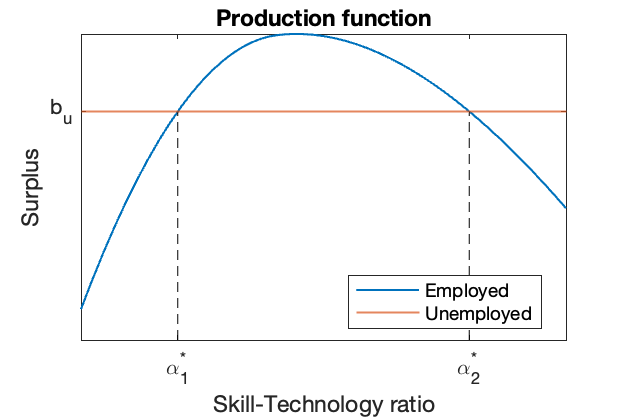
\includegraphics[width=\textwidth]{Analytical1}
\end{figure}

Given $a$, $f(a,b)$ is increasing in $b$ when $b$ is small, then start to decrease in $b$ the mismatch penalty starts to dominate. Given $a$ and $b$, $f(a,b)$ is increasing in $\kappa$ when $b<a$, and decreasing in $\kappa$ when $b>a$. $f(a,b)$ is increasing in $\kappa$ when $b<a$, and decreasing in $\kappa$ when $b>a$. $f(a,b)$ is increasing in $\sigma$. The match is successful when $f(a,b)>b_u$, if $a$ is not too small, then there exists $b_1, b_2$ such that $f(a,b)>b_u$ when $\frac{b}{a} \in (b_1,b_2)$. \\

Apply Taylor expansion to $g(a,b)$: 
\begin{align*}
g(a,b) \approx \kappa a+(1-\kappa) b-\frac{\kappa(1-\kappa)}{2\sigma}\frac{(b-a)^2}{a}+O((b-a)^3)
\end{align*}

In order to have the approximation error bounded, we need $\alpha_o>1$ and $\alpha_u>1$, so that
\begin{align*}
\frac{(b-a)^n}{(\kappa a+(1-\kappa) b)a^{n-1}}<1, &\quad\forall n 
\end{align*}

The lower and upper bound $b_1(a)$ and $b_2(a)$ can be approximated as: 
\begin{align*}
b_1(a) &=\frac{2\alpha_o+(1-\kappa)-\sqrt{4\alpha_o+(1-\kappa)^2}}{2\alpha_o} \\
b_2(a) &=\frac{2\alpha_u+(1-\kappa)+\sqrt{4\alpha_u+(1-\kappa)^2}}{2\alpha_u} \\
\end{align*}

The optimal $b^{*}(a)$ if technology adjustment cost is 0 could be approximated as:
\begin{align*}
b^{*}(a) = \frac{1-\kappa+\alpha_u}{2\alpha_u}a
\end{align*}

The match would be successful ($f(a,b)>b_u$) if $\frac{b}{a}$ falls between $b_1$ and $b_2$. The lower bound $b_1$ is decreasing in $\kappa$ but increasing in $\alpha_o$; while the upper bound $b_2$ is increasing in $\kappa$ but decreasing in $\alpha_u$. The optimal technology level $b^{*}(a)$ is decreasing in $\kappa$ and $\alpha_u$. \\

\subsection{Value of vacancy}
To simplify, I assume that unemployment benefit $b_u = 0$. Also, since $\lambda$ only affect the value of surplus function without changing the decision rule, I assume that $\lambda_n \to \infty$. Then $V_u = V_n = 0$ and $S(a,b)$ can be written as: 
\begin{align*}										
S(a,b)
&= \begin{dcases}
0 & ,f(a,b) \leq 0 \\
\frac{f(a,b)}{1-(1-\delta)\beta} & ,f(a,b)>0
\end{dcases}
\end{align*}
In order to solve the expected value of vacancy, assume that there is no on the job search $s = 0$. $a$ and $b$ are drawn from Pareto distribution. Also assume that skill variance is higher than technology variance, $\lambda_b>\lambda_a>2$:
\begin{align*}
a &\sim Pareto(H,\lambda_a), \quad E(a) = \frac{\lambda_a}{\lambda_a-1}H, \quad var(a) =  \frac{\lambda_a}{(\lambda_a-1)^2(\lambda_a-2)}H^2 \\
b &\sim Pareto(q,\lambda_b), \quad E(b) = \frac{\lambda_b}{\lambda_b-1}Q, \quad var(b) =  \frac{\lambda_b}{(\lambda_b-1)^2(\lambda_b-2)}Q^2
\end{align*}
The expected value of vacancy can be written as: 
\begin{align*}
\Omega_u &= \frac{1}{1-(1-\delta)\beta}\int_a\int_b\Big(f(a,b)-d(a,b)\Big)1\{f(a,b)>0\}d\Gamma_a(a)d\Gamma_b(b) \\
				&= \frac{1}{1-(1-\delta)\beta}\int_a\int_b\Big(g(a,b)-p(a,b)-d(a,b)\Big)1\{f(a,b)>0\}d\Gamma_a(a)d\Gamma_b(b) \\
&=\frac{1}{1-(1-\delta)\beta}\Big(Eg(a,b)-Ep(a,b)-Ed(a,b)\Big)
\end{align*}
Mismatch unemployment measured as the ratio of unsuccessful match can be written as: 
\begin{align*}
M &= \int_a\int_bf(a,b)1\{f(a,b) \leq 0\}d\Gamma_a(a)d\Gamma_b(b)=Em(a,b)
\end{align*}

When $Q$ and $H$ are not too different $b_1<\frac{Q}{H}<b_2$, the expected value of vacancy could be approximated as following: 
\begin{align*}
Eg(a,b) &= \kappa(\frac{\lambda_a}{\lambda_a-1}H)+(1-\kappa)(\frac{\lambda_b}{\lambda_b-1}Q)-\frac{\kappa(1-\kappa)}{2\sigma}\Big(\frac{\lambda_a\lambda_b}{(\lambda_a+1)(\lambda_b-2)}\frac{Q^2}{H}-\frac{2\lambda_b}{\lambda_b-1}Q+\frac{\lambda_a}{\lambda_a-1}H\Big) \\
&-\frac{\lambda_a\lambda_b}{\lambda_a+\lambda_b-1}H(\frac{b_1H}{Q})^{\lambda_a-1}\Big(\frac{\kappa}{\lambda_a-1}+\frac{1-\kappa}{\lambda_a}-\frac{\kappa(1-\kappa)}{2\sigma}(\frac{b_1^2}{\lambda_a+1}-\frac{2b_1}{\lambda_a}+\frac{1}{\lambda_a-1})\Big) \\
&-\frac{\lambda_a\lambda_b}{\lambda_a+\lambda_b-1}H(\frac{b_2H}{Q})^{-\lambda_b}\Big(\frac{\kappa}{\lambda_b}+\frac{1-\kappa}{\lambda_b-1}-\frac{\kappa(1-\kappa)}{2\sigma}(\frac{b_2^2}{\lambda_b-2}-\frac{2b_2}{\lambda_b-1}+\frac{1}{\lambda_b})\Big)
\end{align*}
\begin{align*}
Ep(a,b) = \alpha_u\frac{\lambda_a\lambda_b}{\lambda_a+\lambda_b-1}H(\frac{H}{Q})^{-\lambda_b}\Big(\frac{1}{\lambda_b-2}-\frac{2}{\lambda_b-1}+\frac{1}{\lambda_b}-(\frac{b_2^{-\lambda_b+2}}{\lambda_b-2}-\frac{2b_2^{-\lambda_b+1}}{\lambda_b-1}+\frac{b_2^{-\lambda_b}}{\lambda_b})\Big) \\
Ed(a,b) = \alpha_o\frac{\lambda_a\lambda_b}{\lambda_a+\lambda_b-1}H(\frac{H}{Q})^{\lambda_a-1}\Big(\frac{1}{\lambda_a-1}-\frac{2}{\lambda_a}+\frac{1}{\lambda_a+1}-(\frac{b_1^{\lambda_a-1}}{\lambda_a-1}-\frac{2b_2^{\lambda_a}}{\lambda_a}+\frac{b_2^{\lambda_a+1}}{\lambda_a+1})\Big) \\
\end{align*}
The expected value of vacancy $\Omega_u$ is decreasing in the penalty $\alpha_u$ and $\alpha_o$, and decreasing in the skill and technology dispersion (increasing in $\lambda_a$ and $\lambda_b$). Higher $\kappa$ increases the overqualification penalty while decreases the underqualification penalty. \\

Mismatch unemployment measured as the ratio of unsuccessful match could be approximated as: 
\begin{align*}
Em(a,b) &= \int_a\int_b 1\{f(a,b) \leq 0\}d\Gamma_a(a)d\Gamma_b(b) \\
&= \frac{1}{\lambda_a+\lambda_b}\big(\lambda_b(\frac{b_1H}{Q})^{\lambda_a}+\lambda_a(\frac{b_2H}{Q})^{-\lambda_b}\big)
\end{align*}

Mismatch $M$ is increasing in the return to labor $\kappa$ and the penalty $\alpha_u$ and $\alpha_o$, and increasing in the skill and technology dispersion (increasing in $\lambda_a$ and $\lambda_b$). Mismatch is increasing in $\frac{Q}{H}$ when $\frac{Q}{H}>(b_1^{\lambda_a}b_2^{\lambda_b})^{\frac{1}{\lambda_a+\lambda_b}}$, and decreasing in $\frac{Q}{H}$ when $\frac{Q}{H}<(b_1^{\lambda_a}b_2^{\lambda_b})^{\frac{1}{\lambda_a+\lambda_b}}$. 

\subsection{Optimal skill and technology adoption}
\subsubsection*{Schooling and Innovation (Ex-ante skill and technology adoption)} 
Workers newly entering the market can decide the level of education, which determines the skill level of the distribution they will draw their skill level from. If the skill level they choose $H^*$ is different from the current skill level $H$, they will have to pay a cost convex in the difference $\phi_H(H^*-H)^2/H$. Similarly, new firms are able to invest in R\&D to decide the aggregate technology level of the distribution they will draw their technology level from. If the technology level they choose is different from the current technology level, they will need to pay a cost convex in the difference $\phi_Q(Q^*-Q)^2/Q$. \\

The optimal skill and technology level can be solved by taking first order condition: 
\begin{align*}
\frac{dEg(a,b)}{dH^*}-\frac{dEp(a,b)}{dH^*}-\frac{dEd(a,b)}{dH^*} =2\phi_H(\frac{H^*}{H}-1) \\
\frac{dEg(a,b)}{dQ^*}-\frac{dEp(a,b)}{dQ^*}-\frac{dEd(a,b)}{dQ^*} =2\phi_Q(\frac{Q^*}{Q}-1)
\end{align*}

To solve the optimal technology choice of the firms and the optimal schooling choice of the workers, taking derivative of the expected output and the penalty: 
\begin{align*}
\frac{dEg(a,b)}{dEa} &= \kappa+\frac{\kappa(1-\kappa)}{2\sigma}\Big(\frac{(\lambda_a-1)\lambda_b}{(\lambda_a+1)(\lambda_b-2)}(\frac{Q}{H})^2-1\Big) \\
&-\frac{\lambda_a\lambda_b}{\lambda_a+\lambda_b-1}(\lambda_a-1)(\frac{b_1H}{Q})^{\lambda_a-1}\Big(\frac{\kappa}{\lambda_a-1}+\frac{1-\kappa}{\lambda_a}-\frac{\kappa(1-\kappa)}{2\sigma}(\frac{b_1^2}{\lambda_a+1}-\frac{2b_1}{\lambda_a}+\frac{1}{\lambda_a-1})\Big) \\
&+\frac{(\lambda_a-1)(\lambda_b-1)}{\lambda_a+\lambda_b-1}\lambda_b(\frac{b_2H}{Q})^{-\lambda_b}\Big(\frac{\kappa}{\lambda_b}+\frac{1-\kappa}{\lambda_b-1}-\frac{\kappa(1-\kappa)}{2\sigma}(\frac{b_2^2}{\lambda_b-2}-\frac{2b_2}{\lambda_b-1}+\frac{1}{\lambda_b})\Big) \\
\frac{dEg(a,b)}{dEb} &= (1-\kappa)+\frac{\kappa(1-\kappa)}{2\sigma}\Big(\frac{\lambda_a(\lambda_b-1)}{(\lambda_a+1)(\lambda_b-2)}\frac{2Q}{H}-2\Big) \\
&+\frac{(\lambda_a-1)(\lambda_b-1)}{\lambda_a+\lambda_b-1}\frac{\lambda_a}{b_1}(\frac{b_1H}{Q})^{\lambda_a}\Big(\frac{\kappa}{\lambda_a-1}+\frac{1-\kappa}{\lambda_a}-\frac{\kappa(1-\kappa)}{2\sigma}(\frac{b_1^2}{\lambda_a+1}-\frac{2b_1}{\lambda_a}+\frac{1}{\lambda_a-1})\Big) \\
&-\frac{\lambda_a\lambda_b}{\lambda_a+\lambda_b-1}\frac{\lambda_b-1}{b_2}(\frac{b_2H}{Q})^{-\lambda_b+1}\Big(\frac{\kappa}{\lambda_b}+\frac{1-\kappa}{\lambda_b-1}-\frac{\kappa(1-\kappa)}{2\sigma}(\frac{b_2^2}{\lambda_b-2}-\frac{2b_2}{\lambda_b-1}+\frac{1}{\lambda_b})\Big)
\end{align*}
\begin{align*}
\frac{dEp(a,b)}{dEa} &= -\alpha_u\frac{(\lambda_a-1)(\lambda_b-1)}{\lambda_a+\lambda_b-1}\lambda_b(\frac{H}{Q})^{-\lambda_b}\Big(\frac{1}{\lambda_b-2}-\frac{2}{\lambda_b-1}+\frac{1}{\lambda_b}-(\frac{b_2^{-\lambda_b+2}}{\lambda_b-2}-\frac{2b_2^{-\lambda_b+1}}{\lambda_b-1}+\frac{b_2^{-\lambda_b}}{\lambda_b})\Big) \\
\frac{dEp(a,b)}{dEb} &= \alpha_u\frac{\lambda_a\lambda_b}{\lambda_a+\lambda_b-1}(\lambda_b-1)(\frac{H}{Q})^{-\lambda_b+1}\Big(\frac{1}{\lambda_b-2}-\frac{2}{\lambda_b-1}+\frac{1}{\lambda_b}-(\frac{b_2^{-\lambda_b+2}}{\lambda_b-2}-\frac{2b_2^{-\lambda_b+1}}{\lambda_b-1}+\frac{b_2^{-\lambda_b}}{\lambda_b})\Big) \\
\frac{dEd(a,b)}{dEa} &= \alpha_o\frac{\lambda_a\lambda_b}{\lambda_a+\lambda_b-1}(\lambda_a-1)(\frac{H}{Q})^{\lambda_a-1}\Big(\frac{1}{\lambda_a-1}-\frac{2}{\lambda_a}+\frac{1}{\lambda_a+1}-(\frac{b_1^{\lambda_a-1}}{\lambda_a-1}-\frac{2b_2^{-\lambda_a}}{\lambda_a}+\frac{b_2^{-\lambda_a-1}}{\lambda_a+1})\Big) \\
\frac{dEd(a,b)}{dEb} &=  -\alpha_o\frac{(\lambda_a-1)(\lambda_b-1)}{\lambda_a+\lambda_b-1}\lambda_a(\frac{H}{Q})^{\lambda_a}\Big(\frac{1}{\lambda_a-1}-\frac{2}{\lambda_a}+\frac{1}{\lambda_a+1}-(\frac{b_1^{\lambda_a-1}}{\lambda_a-1}-\frac{2b_2^{-\lambda_a}}{\lambda_a}+\frac{b_2^{-\lambda_a-1}}{\lambda_a+1})\Big) 
\end{align*}
The marginal gain of schooling is increasing in $\frac{Q}{H}$, $\kappa$ and $\alpha_u$, but decreasing in $\alpha_o$; the marginal gain of innovation is decreasing in $\frac{Q}{H}$, $\kappa$ and $\alpha_u$, but increasing in $\alpha_o$. The marginal gain for each production factor is higher when this factor is left behind; the mismatch penalty associated with this lag amplifies the incentive of adjustment.  \\

The optimal growth rate for skill level $\frac{H^*-H}{H}$ is increasing in $\frac{Q}{H}$, $\kappa$ and $\alpha_u$, but decreasing in $\alpha_o$; The optimal growth rate for technology level $\frac{Q^*-Q}{Q}$  is decreasing in $\frac{Q}{H}$, $\kappa$ and $\alpha_u$, but increasing in $\alpha_o$. \\

\subsubsection*{Training and Technology Adoption (Ex-post skill and technology adoption)} 
Consider the technology adoption decision for firms while keeping the skill level unchanged. Once the match is formed, the worker and the firm have the chance to adjust their skill or technology level for the match. The adjustment is a convex function of the adjustment level, the worker needs to pay $\phi_a(a'-a)^2/a$, while the firm needs to pay $\phi_b(b'-b)^2/b$. \\

To have the optimization problem well defined, we need to assume that 
\begin{align*}
\alpha_u &\geq \alpha_o \geq \frac{1}{2}\kappa \\
\alpha_u &\geq \alpha_o \geq \frac{1}{2}(1-\kappa)
\end{align*}

The optimal skill level of the worker could be solved as: 
\begin{align*}
a^*(a,b) &\approx \arg\max_{a'} \tilde{f}_a(a',a,b) \\
\tilde{f_a}(a',a,b)&=\kappa a'+(1-\kappa) b-\alpha_u\frac{(b-a')^2}{b}\1\{b>a'\}-\alpha_o\frac{(a'-b)^2}{a}\1\{a'>b\}-\phi_a\frac{(a'-a)^2}{a} \\
a^*(a,b) 
&= \begin{dcases}
a, \quad \frac{b}{a}<\frac{-\frac{1}{2}\kappa+\alpha_o}{\alpha_o} \\
\frac{\phi_a+\frac{1}{2}\kappa+\alpha_o\frac{b}{a}}{\phi_a+\alpha_o}a, \quad \frac{-\frac{1}{2}\kappa+\alpha_o}{\alpha_o}\leq\frac{b}{a}<\frac{\frac{1}{2}\kappa+\phi_a}{\phi_a} \\
\frac{\phi_a+\frac{1}{2}\kappa+\alpha_u\frac{b}{a}}{\phi_a+\alpha_u}a, \quad \frac{b}{a}\geq\frac{\frac{1}{2}\kappa+\phi_a}{\phi_a}
\end{dcases} 
\end{align*}

The optimal technology level of the firm could be solved as: 
\begin{align*}
b^*(a,b) &\approx \arg\max_{b'} \tilde{f}_b(b',a,b) \\
\tilde{f_b}(b',a,b)&=\kappa a+(1-\kappa) b'-\alpha_u\frac{(b'-a)^2}{b}\1\{b'>a\}-\alpha_o\frac{(a-b')^2}{a}\1\{a>b'\}-\phi_b\frac{(b'-b)^2}{b} \\
b^*(a,b) 
&= \begin{dcases}
\frac{\phi_b+\frac{1}{2}(1-\kappa)+\alpha_o}{\phi_b+\alpha_o\frac{b}{a}}b, \quad \frac{b}{a}<\frac{\phi_b}{\frac{1}{2}(1-\kappa)+\phi_b}\\
\frac{\phi_b+\frac{1}{2}(1-\kappa)+\alpha_u}{\phi_b+\alpha_u\frac{b}{a}}b, \quad \frac{\phi_b}{\frac{1}{2}(1-\kappa)+\phi_b}\leq\frac{b}{a}\leq\frac{\alpha_u}{-\frac{1}{2}(1-\kappa)+\alpha_u}  \\
b, \quad \frac{b}{a} >\frac{\alpha_u}{-\frac{1}{2}(1-\kappa)+\alpha_u}
\end{dcases} 
\end{align*}

The Nash Equilibrium of the match could be solve as: 
\begin{align*}
(a^*(a,b),b^*(a,b))&\approx \arg\max_{a',b'} \tilde{f}_{a,b}(a',b',a,b) \\
\tilde{f}_{a,b}(a',b',a,b)&=\kappa a'+(1-\kappa) b'-\alpha_u(b'-a')^2\1\{b'>a\}-\alpha_o(a'-b')^2\1\{a>b'\} \\
								&-\phi_a\frac{(a'-a)^2}{a}-\phi_b\frac{(b'-b)^2}{b} \\
(a^*(a,b),b^*(a,b)) 
&= \begin{dcases}
(r_1^a(\frac{b}{a})a,r_1^b(\frac{b}{a})b), \quad  \frac{b}{a}< \alpha_1\\
(r_2^a(\frac{b}{a})a,r_2^b(\frac{b}{a})b), \quad \alpha_1 \leq \frac{b}{a} < \alpha_2\\
(r_3^a(\frac{b}{a})a,r_3^b(\frac{b}{a})b), \quad \alpha_2 \leq \frac{b}{a} < \alpha_3 \\
(r_4^a(\frac{b}{a})a,r_4^b(\frac{b}{a})b), \quad  \frac{b}{a} \geq \alpha_3
\end{dcases} 
\end{align*}
With the growth rate and threshold defined as following: 
\begin{align*}
&r_1^a(\frac{b}{a}) = 1 , && r_1^b(\frac{b}{a}) = \frac{\phi_b+\frac{1}{2}(1-\kappa)+\alpha_o}{\phi_b+\alpha_o\frac{b}{a}} \\
&r_2^a(\frac{b}{a}) = \frac{\phi_a+\frac{1}{2}\kappa+\alpha_o(1+\frac{\phi_a}{\phi_b}+\frac{1}{2\phi_b})\frac{b}{a}}{\phi_a+\alpha_o(1+\frac{\phi_a}{\phi_b}\frac{b}{a})} , && r_2^b(\frac{b}{a}) = \frac{\phi_b+\frac{1}{2}(1-\kappa)+\alpha_o(1+\frac{\phi_b}{\phi_a}+\frac{1}{2\phi_a})}{\phi_b+\alpha_o(\frac{b}{a}+\frac{\phi_b}{\phi_a})} \\
&r_3^a(\frac{b}{a}) = \frac{\phi_a+\frac{1}{2}\kappa+\alpha_u(1+\frac{\phi_a}{\phi_b}+\frac{1}{2\phi_b})\frac{b}{a}}{\phi_a+\alpha_u(1+\frac{\phi_a}{\phi_b}\frac{b}{a})} , && r_3^b(\frac{b}{a}) = \frac{\phi_b+\frac{1}{2}(1-\kappa)+\alpha_u(1+\frac{\phi_b}{\phi_a}+\frac{1}{2\phi_a})}{\phi_b+\alpha_u(\frac{b}{a}+\frac{\phi_b}{\phi_a})} \\
&r_4^a(\frac{b}{a}) = \frac{\phi_a+\frac{1}{2}\kappa+\alpha_u\frac{b}{a}}{\phi_a+\alpha_u}, && r_4^b(\frac{b}{a}) =  1 
\end{align*}

\begin{align*}
\alpha_1 =  \frac{\alpha_o\phi_b-\frac{1}{2}\kappa\phi_b}{\alpha_o(\phi_b+\frac{1}{2})}, \quad \alpha_2 = \frac{\phi_a\phi_b+\frac{1}{2}\kappa\phi_b}{\phi_a\phi_b+\frac{1}{2}(1-\kappa)\phi_a}, \quad \alpha_3 =  \frac{\frac{1}{2}(1-\kappa)\phi_a+\alpha_u(\phi_a+\frac{1}{2})}{\alpha_u\phi_a} \\
\end{align*}

The limit of growth rate for each match could be solved: 
\begin{align*}
&r_1^a(\frac{b}{a}) = 1 , &&  r_1^b(\frac{b}{a}) \in [\frac{\phi_b+\frac{1}{2}}{\phi_b},\frac{\phi_b+\frac{1}{2}(1-\kappa)+\alpha_o}{\phi_b}]\\
&r_2^a(\frac{b}{a}) \in [1,\frac{\phi_a+\frac{1}{2}\kappa}{\phi_a}) , &&  r_2^b(\frac{b}{a}) \in [\frac{\phi_b+\frac{1}{2}(1-\kappa)}{\phi_b},\frac{\phi_b+\frac{1}{2}}{\phi_b})\\
&r_3^a(\frac{b}{a})  \in [\frac{\phi_a+\frac{1}{2}\kappa}{\phi_a},\frac{\phi_a+\frac{1}{2}}{\phi_a}) , && r_3^b(\frac{b}{a}) \in [1,\frac{\phi_b+\frac{1}{2}(1-\kappa)}{\phi_b})\\
&r_4^a(\frac{b}{a}) \in [\frac{\phi_a+\frac{1}{2}}{\phi_a}, \frac{\phi_a+\frac{1}{2}\kappa+\alpha_u}{\phi_a}],  && r_4^b(\frac{b}{a}) = 1 
\end{align*}

\subsection{Growth path}
Assume that $\phi_H \to \infty$, $\phi_b \to \infty$ and $\lambda_b \to \infty$. The firms can enter the market by choosing their technology level without uncertainty, workers will adjust their skill level after being matched to the firm. \\

The initial technology level is given as $Q_0$, the initial skill distribution follows Pareto distribution with lower bound $H_0 = \frac{Q_0}{b_1}$ and dispersion parameter $\lambda_a$. Initially, there is no mismatch in this economy, all the matches will be formed successfully. Here, we start with the case where $f_u=1$ and $\delta=1$, all the workers eligible to work will be matched to the firm, and the match will breakup at the end of the period. \\

At each period, the workers with successful match will follow the policy solved above, given a sequence of technology chosen by firm, the skill distribution will evolve as following: 
\begin{align*}
F_{t+1}(a)
&= \begin{dcases}
F_t(a),\quad  a \leq \frac{1}{b_2}Q_{t+1} \\
F_t(\frac{1}{b_2}Q_{t+1}),\quad  \frac{1}{b_2}Q_{t+1}< a \leq (\frac{\rho_u}{b_2}+\tau_u)Q_{t+1} \\
F_t(\frac{a-\tau_uQ_t}{\rho_u}), \quad (\frac{\rho_u}{b_2}+\tau_u)Q_{t+1}< a \leq \frac{\phi_a}{\phi_a+\frac{1}{2}\kappa}Q_{t+1} \\
F_t(\frac{a-\tau_oQ_t}{\rho_o}),  \quad \frac{\phi_a}{\phi_a+\frac{1}{2}\kappa}Q_{t+1}<a \leq \frac{\alpha_o}{\alpha_o-\frac{1}{2}\kappa}Q_{t+1} \\
F_t(a), \quad a>\frac{\alpha_o}{\alpha_o-\frac{1}{2}\kappa}Q_{t+1} \\
\end{dcases} \\
\rho_u &= \frac{\frac{1}{2}\kappa+\phi_a}{\alpha_u+\phi_a}, \quad \tau_u = \frac{\alpha_u}{\alpha_u+\phi_a}, \quad
\rho_o = \frac{\frac{1}{2}\kappa+\phi_a}{\alpha_o+\phi_a}, \quad \tau_o = \frac{\alpha_o}{\alpha_o+\phi_a} 
\end{align*}
To simply, consider the case where $\alpha_u = \alpha_o$. 
\begin{figure}[h!]
\centering
\caption{Distribution Evolution: Low Mismatch Penalty}
\label{Analytical2_1}
\includegraphics[width=\textwidth]{Analytical_Growth2_1}
\end{figure}]
\begin{figure}[h!]
\centering
\caption{Distribution Evolution: High Mismatch Penalty}
\label{Analytical2_2}
\includegraphics[width=\textwidth]{Analytical_Growth2_2}
\end{figure}
\begin{align*}
F_{t+1}(a)
&= \begin{dcases}
F_t(a),\quad  a \leq \frac{1}{b_2}Q_{t+1} \\
F_t(\frac{1}{b_2}Q_{t+1}),\quad  \frac{1}{b_2}Q_{t+1}< a \leq (\frac{\rho}{b_2}+\tau)Q_{t+1} \\
F_t(\frac{a-\tau Q_t}{\rho}), \quad (\frac{\rho}{b_2}+\tau)Q_{t+1} < a \leq \gamma Q_{t+1} \\
F_t(a), \quad a>\gamma Q_{t+1} \\
\end{dcases} \\
\rho &= \frac{\frac{1}{2}\kappa+\phi_a}{\alpha_u+\phi_a}, \quad \tau = \frac{\alpha_u}{\alpha_u+\phi_a}, \quad \gamma = \frac{\alpha_u}{\alpha_u-\frac{1}{2}\kappa}
\end{align*}
Workers with skill level below $\frac{Q_t}{b_2}$ would exit the market, since they will never be matched to any firm successfully. As a result, at time $t$, we only need to track the part of the distribution where $a>\frac{Q_t}{b_2}$. \\

Define $I_t(j)$ and $T_t(j,a)$ as following, consider the case where the growth rate of technology is constant $\frac{Q_{t+1}}{Q_t} = R_Q$, then $F_t$ could be expressed in terms of $F_0$. 
\begin{align*}
I_t(j) &= \rho^{t-j}\gamma {Q_j}+\sum_{i=j+1}^t\rho^{t-i}\tau Q_i = \gamma \rho^{t-j}R_Q^jQ_0+(R_Q^{t+1}-R_Q^{j+1}\rho^{t-j})\frac{\tau Q_0}{R_Q-\rho} \\
T_t(j,a) &= \rho^{j-(t+1)}a+\sum_{i=j}^t\rho^{j-(i+1)}\tau Q_i  =  \rho^{j-(t+1)}a+(R_Q^{t+1}\rho^{j-(t+1)}-R_Q^{j})\frac{\tau Q_0}{R_Q-\rho} \\
\end{align*}

When $R_Q<\rho+\tau b_2$, 
\begin{align*}
F_t(a)
&= \begin{dcases}
F_0(\frac{Q_1}{b_2}),\quad  \frac{Q_t}{b_2} \leq I_t(1)  \\
F_0(T_t(j,a)), \quad I_t(j-1)\leq a < I_t(j), \quad 1 \leq j \leq t\\
F_0(a), \quad  a>\gamma Q_t \\
\end{dcases} \\
I_t(0) &= \rho^t\frac{Q_1}{b_2}+\sum_{i=1}^t\rho^{t-i}\tau Q_i = \rho^t\frac{Q_1}{b_2}+(R_Q^t-\rho^t)\frac{R_Q}{R_Q-\rho}\tau Q_0
\end{align*}

When $\rho+\tau b_2 \leq R_Q <\gamma b_2$,
\begin{align*}
F_t(a)
&= \begin{dcases}
F_0(T_{t-1}(t-1,\frac{Q_t}{b_2})),\quad  \frac{Q_t}{b_2} \leq I_t(1)  \\
F_0(T_t(j,a)), \quad I_t(j-1)\leq a < I_t(j), \quad 1 \leq j \leq t\\
F_0(a), \quad  a>\gamma Q_t \\
\end{dcases} \\
I_t(0) &= (\frac{\rho}{b_2}+\tau)Q_t
\end{align*}

When $R_Q \geq \gamma b_2$, 
\begin{align*}
F_t(a)
&= \begin{dcases}
F_0(\frac{Q_t}{\rho b_2}),\quad  \frac{Q_t}{b_2} \leq a <(\frac{\rho}{b_2}+\tau)Q_t  \\
F_0(\frac{a}{\rho}-\frac{\tau Q_t}{\rho}), \quad (\frac{\rho}{b_2}+\tau)Q_t  \leq a < \gamma Q_t \\
F_0(a), \quad  a>\gamma Q_t \\
\end{dcases} \\
\end{align*}
The mismatch level of the economy is defined as the ratio of workers who will never be matched to the firm: 
\begin{align*}
M_t &= F_t(\frac{Q_t}{b_2}) \\
&= \begin{dcases}
1-R_Q^{-\lambda_a}, \quad R_Q \leq \rho+\tau b_2 \\
1-\rho^{\lambda_a}(R_Q^t+\frac{R_Q^t-R_Q^{t-1}\rho}{R_Q-\rho}\tau b_2)^{-\lambda_a} \quad \rho+\tau b_2 \leq R_Q <\gamma b_2 \\
1-(R_Q^t)^{-\lambda_a}, \quad R_Q> \gamma b_2
\end{dcases} 
\end{align*}
\subsection{Labor market trend}
In Acemoglu and Autor(2011)\cite{AcemogluAutor2011}, they documented the labor market trend in terms of the wage and employment distribution. At the early phase, all the wage levels grow at similar rate, then the low wage group starts to experience a wage drop; in the recent years, low wage group starts to catch up, not only in wage level but also in employment. 
\begin{figure}[h!]
\centering
\caption{Wage Trend}
\label{Wage1}
\includegraphics[width=\textwidth]{Wage3}
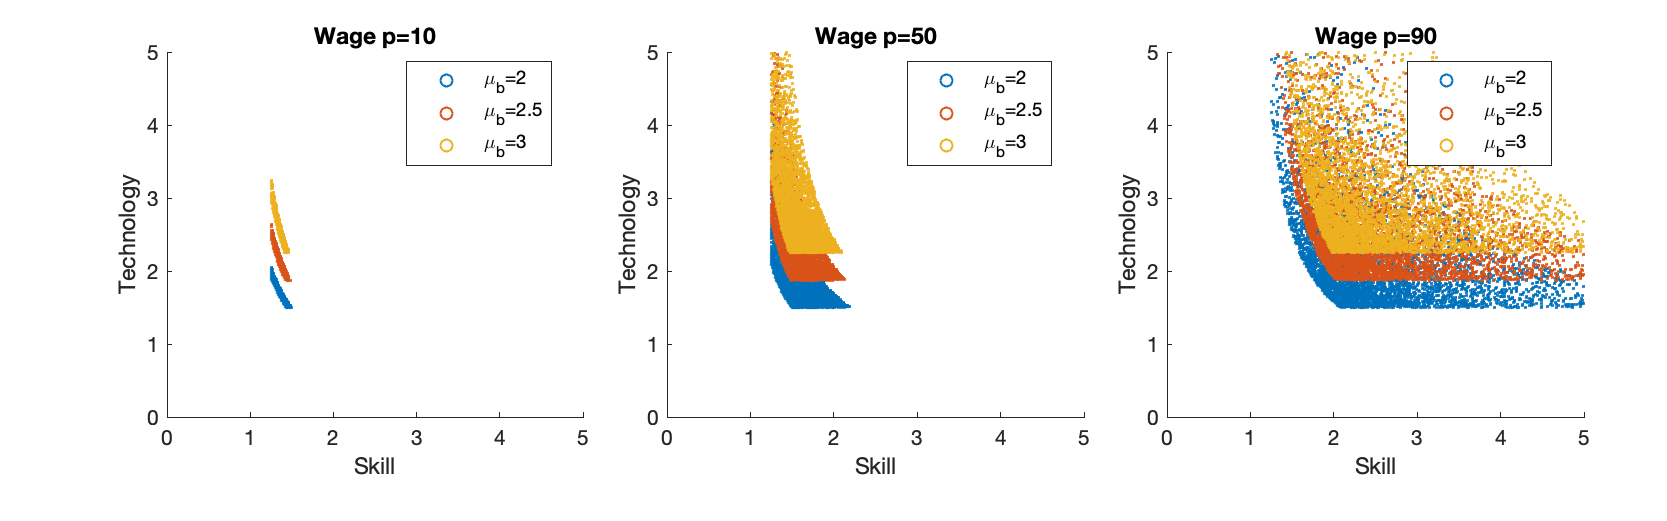
\includegraphics[width=\textwidth]{Task3}
\includegraphics[width=\textwidth]{Wage1}
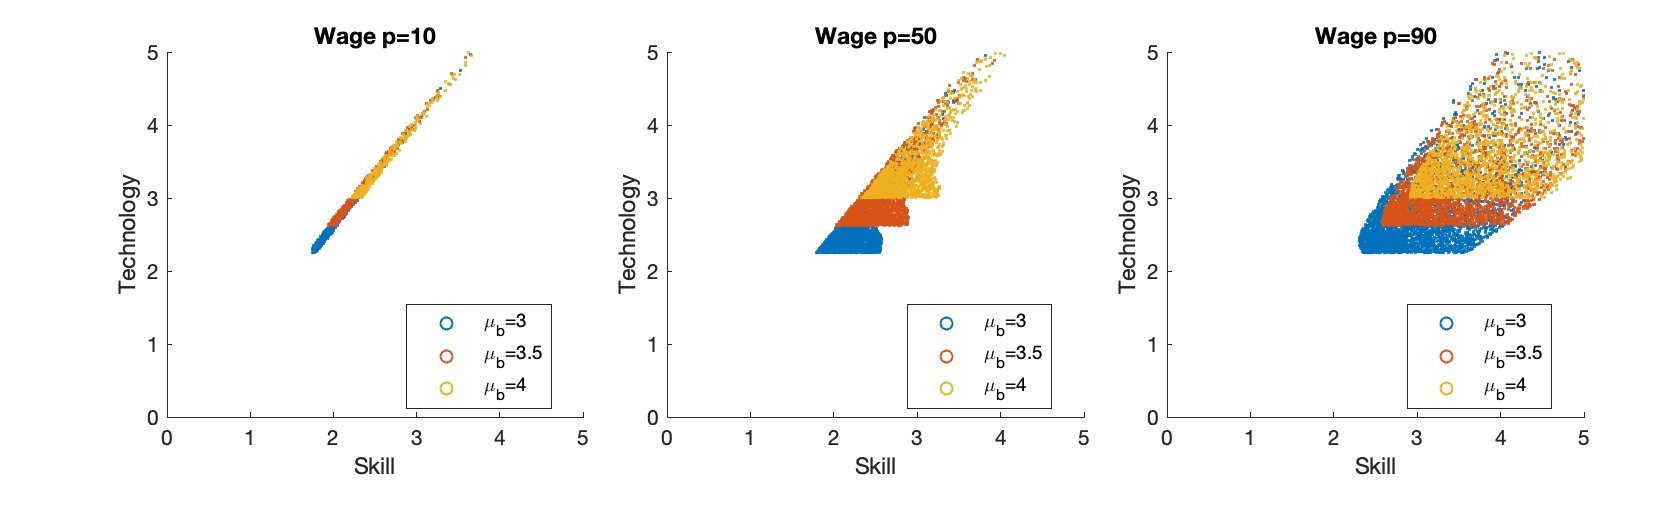
\includegraphics[width=\textwidth]{Task1}
\end{figure}

\begin{figure}[h!]
\centering
\caption{Marginal return to technology}
\label{Wage1}
\includegraphics[width=\textwidth]{Wage_Skill}
\end{figure}

The simulation result of the benchmark model is shown in figure \ref{Wage1}. When the technology level is low, the productivity effects would dominate with an increase of technology, all the wage group level will experience a wage increase. Low skill workers benefit from the productivity gain, which dominates the mismatch penalty; high skill workers can benefit from reducing the over-qualification disutility. When the technology level continue to increase, the mismatch term would play an important effect for the low wage group, the wage level for the low wage group will decrease; but the productivity effect would still dominate for the high wage group, so their wage level will continue to increase. As a result, at this stage, the wage gap or skill premium would increase. When the technology level keep increasing, the lowest skilled workers will exit the market, the wage level of the low wage group starts to catch up, since the low wage position has now changed, the skill level of workers for the low wage group has increased. 


\clearpage
\bibliographystyle{plain}
\bibliography{Mismatch}

\clearpage
\section{Variable list}
\begin{longtable}{ll}
\hline \hline
Letter     &       Description                          \\
\hline 
$\rho_z, \sigma_z$  &  AR(1) process for log TFP \\
$a_i$                 & Worker $i$'s skill level                       \\
$\rho_b, \sigma_b$  &  Skill distribution\\
$b_j$                &  Firm $j$'s technology level                \\
$\rho_b, \sigma_b$  &  Technology distribution\\
$s$ & OJS efficiency \\
$\Phi$ & Matching efficiency \\
$\alpha$ & Matching function elasticity \\
$\phi$ & Job arriving rate \\
$\sigma$ & Elasticity of substitution between technology and skill \\
$b_u$ & Unemployment benefit \\
$\delta$ & Exogenous separation rate \\
$\delta_a$ & Human capital depreciation rate \\
$\delta_b$ & Technology depreciation rate \\
\hline 
\end{longtable}
\end{document}
